\documentclass[11pt]{article}

\usepackage[a4paper, margin=1in]{geometry}
\usepackage[T1]{fontenc}
\usepackage[utf8]{inputenc}
\usepackage{amsmath, amssymb}
\usepackage{booktabs}
\usepackage{graphicx}
\usepackage{hyperref}
\usepackage{xcolor}
\hypersetup{colorlinks=true, linkcolor=blue, urlcolor=blue, citecolor=blue}
\usepackage{authblk}
\usepackage{microtype}
\usepackage{enumitem}
\setlist[itemize]{leftmargin=1.4em}

\title{Quantum Mechanics as Multiphase 3D Continuum Mechanics \\[0.2em]
\large Realised through Mind--AI Cooperation \\[0.3em]
\normalsize\textit{Version 3: wave-function formulation of the mathematical model}}

\author[1]{Claes Johnson}
\affil[1]{KTH Royal Institute of Technology, Stockholm, Sweden \\
\texttt{claesjohnson@gmail.com}}
\date{\today \\[0.5em]
\textit{This article was written by Claude (Anthropic) with assistance by the author.} \\
\textit{The mathematical theory and the simulation framework are the author's;} \\
\textit{the implementation was developed by Claude from p5.js prototypes by the author.}}

\begin{document}
\maketitle

\begin{abstract}
We present a formulation of the $N$-electron quantum-mechanical model in terms of a wave function $\Psi(\mathbf{x}) = \sum_{i=1}^{N} \psi_i(\mathbf{x})$ defined over physical 3D space with coordinate $\mathbf{x} \in \mathbb{R}^3$, with the $\psi_i$ unit-charge individual electronic wave functions with supports in a non-overlapping decomposition of $\mathbb{R}^3$ into domains $\Omega_i$ with boundaries $\Gamma_i = \partial \Omega_i$. An atomic or molecular ground state is determined by minimization of the standard Coulomb energy functional over the wave functions $\{\psi_i\}$ and over the domain decomposition $\{\Omega_i\}$, subject to continuity of $\Psi$ across the common inter-domain boundaries $\Gamma_i \cap \Gamma_j$. The minimum is approached by a gradient method with three coupled updates: imaginary-time propagation of each $\psi_i$, Poisson updates of the per-electron Hartree potentials, and level-set updates of the free boundary of the domain decomposition $\{\Omega_i\}$. We refer to this real-space formulation as \textbf{RealQM}.

The model is organised as a hierarchy of reductions: \textbf{Level 1} is the parameter-free basic atomic model in which shell structure emerges from minimum-energy packing rather than being preset, reproducing observed atom total energies for elements Li--Rn within ${\sim}1\%$; \textbf{Level 2} treats atoms with spherical symmetry on the inner shells while leaving valence electrons explicit; \textbf{Level 3} replaces nucleus and inner shells together by a pseudo-kernel characterised by an effective charge and a softening radius; \textbf{Level 4} assembles Level-3 atoms into molecules and molecular complexes. At Level 3, reduced-kernel architectures sweep entire periodic-table columns --- closed-shell hydrides match experimental atomization energies within 3--9\% for groups 1, 2, 14, and 16 (NaH, BeH$_2$, H$_2$O, CH$_4$, SiH$_4$, GeH$_4$); the H$_2$ covalent bond at parameter-free Level 1 matches Kolos--Wolniewicz to 0.3\% on total energy and the experimental dissociation energy to 3\%. Reactive chemistry (proton transfer, exchange) and excited states (orthohelium) follow from the same variational principle. At Level 4, the framework supports \textbf{interactive protein folding}: polyglycine hairpins fold from extended to compact via quantum-mechanical H-bond forces alone; alpha-helices form from near-linear chains; mini-proteins fold under universal $i \to i{+}4$ H-bond bias plus a single hydrophobic-pressure parameter, reproducing native-like topology without empirical force fields. A three-system condensed-phase calibration (NaCl crystal melt, CO$_2$ dry ice, solid N$_2$) shows that the simulation transition T sits in the 1000--2000~K range across systems and that the overshoot factor against experimental phase-transition temperatures scales with the missing-dispersion contribution.

\textbf{Stability of matter} for a system of $N$ non-overlapping atoms with kernel charge $Z$ follows from the Hardy inequality applied to the global wave function $\Psi$ as a one-paragraph derivation, giving the bound $E \ge -C N Z^3$ --- in striking contrast to the Dyson--Lenard--Lieb--Thirring proof required in standard quantum mechanics. The same multiphase formulation extends naturally to atomic nuclei in a proton--electron picture (4 protons + 2 electrons for He-4), demonstrating reach beyond chemistry to nuclear-scale physics.

The framework is implemented in ${\sim}8000$ lines of JavaScript and WebGPU compute shaders running interactively in a browser on a consumer laptop GPU --- three orders of magnitude smaller and ${\sim}10^2$--$10^4 \times$ faster than mainstream quantum-chemistry packages. The implementation, validation suite, and curated public Gallery were developed through extended collaboration with an AI code assistant (Claude, Anthropic) starting from initial p5.js prototypes by the author. We present the collaboration as part of the contribution: a worked case of how a single mathematical mind, paired with an AI engineering partner, can produce research-grade interactive scientific software at a scale that previously required a programming team.

\medskip
\noindent \textbf{Keywords:} quantum chemistry; multiphase wave functions; free-boundary problems; Bernoulli condition; real-space methods; stability of matter; WebGPU; AI-assisted scientific software; human--AI collaboration.
\end{abstract}

\section{Introduction}

The $N$-electron Schr\"odinger equation has been the foundation of quantum chemistry for nearly a century. In its standard formulation, matter is described as eigenfunctions of an $N$-body Hamiltonian acting on antisymmetric wavefunctions in a $3N$-dimensional configuration space. The exponential scaling of this representation has been mitigated by approximate methods --- Hartree--Fock, density functional theory, configuration interaction, coupled cluster --- each making specific compromises between accuracy and computational cost~\cite{HK64,KS65,MHG17}. Production-quality quantum chemistry packages comprise hundreds of thousands to millions of lines of code, draw on decades of accumulated machinery for basis sets, integral evaluation, and analytic gradients, and require dedicated computational clusters for systems of biological size.

\paragraph{Two foundational positions.}
Two quotations from the founders frame the conceptual position of this paper. The first is from \textbf{Dirac, 1929}, on the relation between physics and chemistry:

\begin{quote}
The underlying physical laws necessary for the mathematical theory of [\ldots] the whole of chemistry are thus completely known, [and] the difficulty is only that the exact application of these laws leads to equations much too complicated to be soluble.
\end{quote}

The second is from \textbf{Schr\"odinger, in a letter to Lorentz dated 6 June 1926}, sketching how he originally intended to interpret the wave function for $N>1$ electrons:

\begin{quote}
If we now have to deal with $N$ particles, then $\Psi(x_1, \ldots, x_N)$ is a function of $N$ variables $x_1, \ldots, x_N$ over $N$ 3D spaces $R_1, \ldots, R_N$. Now first let $R_1$ be identified with the real space $\mathbb{R}^3$ and integrate over $R_2, \ldots, R_N$. Second, identify $R_2$ with the real space and integrate over $R_1, R_3, \ldots, R_N$ and so on. The $N$ individual results are to be added after they have been multiplied by certain constants which characterise the particles. \emph{I consider the result to be the electric charge density in real space.}
\end{quote}

The two positions are complementary. Dirac states that chemistry reduces to known physical laws; the only obstacle is computational. Schr\"odinger sketches a real-space interpretation in which the $N$-electron wave function projects to an actual charge density in physical $\mathbb{R}^3$, recovering the direct physical meaning that $\psi^2$ has for the hydrogen atom. \textbf{This real-space-density interpretation was abandoned during the late 1920s under the dominance of the Bohr--Heisenberg--Dirac Copenhagen interpretation}, in which $\Psi$ on $\mathbb{R}^{3N}$ became a probability amplitude rather than a physical charge density. The resulting Standard QM (StdQM) inherits the computational obstacle Dirac identified --- solving an equation on $3N$-dimensional configuration space --- and the chemistry-specific approximations introduced to make it tractable have, ever since, made chemistry look more autonomous from physics than Dirac's position would suggest.

The formulation developed in this paper, which we call \textbf{RealQM}, returns to the originally proposed real-3D-space picture. The $N$-electron wave function $\Psi(\mathbf{x}) = \sum_{i=1}^N \psi_i(\mathbf{x})$ lives on physical $\mathbb{R}^3$ as a sum of one-electron wave functions $\psi_i$ on non-overlapping spatial domains, with $\psi_i^2$ the actual electron charge density of electron $i$. The $3N$-dimensional configuration-space step is not taken at all; the computational obstacle Dirac identified is dissolved by working in 3D throughout, at the cost of replacing antisymmetry with strict spatial non-overlap.

We treat an $N$-electron system not as a wave function on $\mathbb{R}^{3N}$ configuration space but as a sum $\Psi(\mathbf{x}) = \sum_{i=1}^{N} \psi_i(\mathbf{x})$ of \textbf{one-electron wave functions} $\psi_i$ defined over physical 3D space with coordinate $\mathbf{x} \in \mathbb{R}^3$, where each $\psi_i^2$ is a unit charge density with support in a non-overlapping decomposition of $\mathbb{R}^3$ into domains $\Omega_i$. Energy is the standard Coulomb functional. The minimum is taken over the wave functions $\{\psi_i\}$, over the domain decomposition $\{\Omega_i\}$, and over the nuclear positions; molecular geometry, bonding, and dynamics emerge from the same variational principle.

In this respect RealQM is a direct realisation of \textbf{Dirac's chemistry-as-applied-physics position} (the 1929 quote above) executed in the real-3D-space picture Schr\"odinger originally envisaged. RealQM takes Dirac's program seriously by retaining only the underlying physics --- Coulomb interactions between electronic wave functions and nuclei --- and discarding the chemistry-specific machinery (basis sets, exchange--correlation functionals, fitted force fields) that StdQM had to introduce in order to make the configuration-space equations tractable. Chemistry then re-emerges, bottom-up, from the variational principle alone.

This reformulation --- RealQM in what follows --- is not merely a numerical recasting of the standard problem. It is a different mathematical object with different scaling: complexity grows with the number of mesh points in 3D, not with the number of basis functions in $N \times 3D$. As a consequence, the entire framework can be implemented in roughly 8000 lines of JavaScript and WebGPU compute shaders, runs in a browser on a consumer laptop GPU, and supports interactive simulation of systems with hundreds of explicit electrons in real time.

We organize the model as a hierarchy of reductions. \textbf{Level 1} is parameter-free: an atom is described as a nucleus of charge $Z$ surrounded by $N$ one-electron wave functions $\psi_i$ on non-overlapping shell-shaped domains $\Omega_i$, with the configuration determined by minimum-energy packing. The Level-1 atomic model reproduces observed atom energies for elements Li through Rn to approximately 1\% with no fitted constants. \textbf{Level 2} spherically homogenizes inner shells, keeping the shell occupancy intact but replacing the angular structure of $\sum_{i \in {\rm shell}} \psi_i^2$ with a radial density of matching total charge. \textbf{Level 3} further replaces the nucleus and inner shells together by a \emph{pseudo-kernel} characterized by an effective charge $Z_{\rm kernel}$ and a softening radius $r_c$, leaving only the outermost valence wave functions explicit. \textbf{Level 4} combines Level-3 atoms into molecular assemblies. Each level is determined by comparison with the prior level, in the same architectural spirit as pseudopotentials and frozen-core methods in standard quantum chemistry, but with a parameter-free ab initio bottom rather than empirical fits.

A second contribution of this paper concerns how the implementation was produced. The mathematical reformulation is the work of one author. The validation suite, the WebGPU compute shaders, the systematic kernel-architecture sweeps reported in Section~\ref{sec:validation}, and the curated public Gallery were developed through extended interactive collaboration with \textbf{Claude}, a large-language-model AI assistant produced by Anthropic. The pattern of the collaboration was iterative and recorded: the human proposed mathematical and chemical questions; the AI translated them into runnable simulations, identified bugs, ran systematic parameter sweeps, and challenged claims that did not survive scrutiny; the human evaluated the results and corrected the AI's interpretations when they slipped. The history of corrections --- claims made, retracted, refined, restored --- is itself part of the public record, encoded in the Gallery's ``Assessment by Claude'' card.

We take this case to be a worth-reporting example of how a single mathematical mind, working with an AI engineering partner in real time, can produce research-grade interactive scientific software at a scale otherwise requiring a programming team. The collaboration is not the science, but it is part of how the science came into existence, and we report it as such.

The paper is organized as follows. Section~\ref{sec:reformulation} states the reformulation and the hierarchical reduction. Section~\ref{sec:implementation} describes the numerical implementation. Section~\ref{sec:validation} reports validation, including atom energies, the covalent H$_2$ bond and its He limit, atomization energies of closed-shell hydrides across periodic-table groups, S66 dimer geometries, chemical reactions, protein folding, excited states, and a three-system condensed-phase calibration (NaCl crystal melt, CO$_2$ dry-ice cluster, solid N$_2$) that quantifies how the simulation's overshoot factor against experimental transition temperatures scales with the missing-dispersion contribution. Section~\ref{sec:limitations} states honest limits of the approach. Section~\ref{sec:som} shows that stability of matter --- the lower bound $E \ge -C N Z^2$ on the ground-state energy of a system of $N$ atoms --- follows directly from the Hardy inequality applied to non-overlapping electronic territories, in contrast to the heroic Dyson--Lenard--Lieb--Thirring proof required in standard quantum mechanics. Section~\ref{sec:nucleus} reports an analogous model of the atomic nucleus, demonstrating that the framework extends beyond chemistry to nuclear-scale physics. Section~\ref{sec:chemvphys} places the work in the long-standing chemistry-vs-physics debate. Section~\ref{sec:collaboration} discusses the human--AI collaboration. The full source code, validation suite, and interactive Gallery are available at the URLs in Section~\ref{sec:code}.

\section{RealQM Schr\"odinger Equation}\label{sec:reformulation}

\subsection{Multiphase 3D formulation}

The starting point is Schr\"odinger's 1926 model of the hydrogen atom: a single real-valued wave function $\psi : \mathbb{R}^3 \to \mathbb{R}$, normalised by $\int_{\mathbb{R}^3} \psi^2(\mathbf{x})\,d\mathbf{x} = 1$, with $\psi^2(\mathbf{x})$ representing the electron charge density and the total energy
\begin{equation}\label{eq:H-energy}
E(\psi) = \tfrac{1}{2} \int_{\mathbb{R}^3} |\nabla \psi(\mathbf{x})|^2 \, d\mathbf{x}
\;-\; \int_{\mathbb{R}^3} \frac{\psi^2(\mathbf{x})}{|\mathbf{x}|}\, d\mathbf{x}
\end{equation}
balancing kinetic localisation cost against Coulomb attraction to a unit positive kernel at the origin. The ground state minimises $E(\psi)$ and gives the well-known $E = -1/2$ Ha eigenvalue, in agreement with observation.

For an atomic system with $N>1$ electrons the standard approach (Schr\"odinger 1926, with the non-physical configuration-space step taken on Born--Heisenberg suggestion) is to extend $\psi$ to a wave function $\Psi(\mathbf{x}_1, \ldots, \mathbf{x}_N)$ on $\mathbb{R}^{3N}$, with $\Psi^2$ given a probabilistic interpretation. This step replaces three-dimensional physical space with an $N$-fold tensor product whose computational cost grows exponentially in $N$ and whose physical meaning has been contested ever since.

\textbf{The RealQM alternative} keeps the wave function in physical $\mathbb{R}^3$. The $N$-electron wave function $\Psi \in H^1(\mathbb{R}^3)$ is a sum of one-electron wave functions $\psi_i$ on non-overlapping spatial domains $\Omega_i$:
\begin{equation}\label{eq:Psi-sum}
\Psi(\mathbf{x}) = \sum_{i=1}^{N} \psi_i(\mathbf{x}),
\qquad
\psi_i \in H^1(\Omega_i), \qquad \int_{\Omega_i} \psi_i^2(\mathbf{x})\, d\mathbf{x} = 1,
\end{equation}
where $\{\Omega_i\}_{i=1}^{N}$ is a partition of physical space into open non-overlapping regions, $\Omega_i \cap \Omega_j = \emptyset$ for $i \ne j$, and $H^1(\Omega)$ denotes the space of real-valued functions on $\Omega$ with square-integrable first derivatives. The boundaries $\Gamma_i = \partial \Omega_i$ are not specified in advance: they emerge as a free boundary, with the $\psi_i$ being continuous across joint boundaries $\Gamma_i \cap \Gamma_j$ as imposed by $\Psi \in H^1(\mathbb{R}^3)$, and the boundary location determined by the energy minimisation.

The total energy of $\Psi$ is the sum of three Coulomb contributions:
\begin{equation}\label{eq:TE}
TE(\Psi) = K(\Psi) + PK(\Psi) + PE(\Psi),
\end{equation}
with kinetic-energy term
\begin{equation}\label{eq:K}
K(\Psi) = \tfrac{1}{2} \int_{\mathbb{R}^3} |\nabla \Psi(\mathbf{x})|^2\, d\mathbf{x}
\;=\; \sum_{i=1}^{N} \tfrac{1}{2} \int_{\Omega_i} |\nabla \psi_i(\mathbf{x})|^2\, d\mathbf{x},
\end{equation}
attractive kernel-electron potential energy
\begin{equation}\label{eq:PK}
PK(\Psi) = \int_{\mathbb{R}^3} W(\mathbf{x})\, \Psi^2(\mathbf{x})\, d\mathbf{x},
\qquad
W(\mathbf{x}) = -\sum_{a=1}^{M} \frac{Z_a}{|\mathbf{x} - \mathbf{R}_a|},
\end{equation}
and inter-electron repulsive potential energy without self-repulsion
\begin{equation}\label{eq:PE}
PE(\Psi) = \sum_{i=1}^{N} \int_{\Omega_i} \sum_{j \ne i} V_j(\mathbf{x})\, \psi_i^2(\mathbf{x})\, d\mathbf{x},
\qquad
V_j(\mathbf{x}) = \int_{\Omega_j} \frac{\psi_j^2(\mathbf{y})}{2\,|\mathbf{x} - \mathbf{y}|}\, d\mathbf{y}.
\end{equation}
The exclusion $j \ne i$ in~\eqref{eq:PE} removes self-repulsion by construction, since the regions $\Omega_i, \Omega_j$ are disjoint and each electron contributes its own charge density only to the potentials seen by the other electrons. The nuclear--nuclear Coulomb term $V_{NN}$ is included additively when nuclear positions are varied.

The ground-state configuration is found by minimising~\eqref{eq:TE} over $\Psi = \sum_i \psi_i$ with $\psi_i \in H^1(\Omega_i)$, $\int_{\Omega_i} \psi_i^2 = 1$, and over both the partition $\{\Omega_i\}$ and the nuclear positions $\{\mathbf{R}_a\}$. Variation with respect to $\psi_i$ at fixed $\Omega_i$ gives, with Lagrange multiplier $E_i$ for the unit-norm constraint,
\begin{equation}\label{eq:Hi}
\mathcal{H}_i \psi_i \;\equiv\; \Bigl(-\tfrac{1}{2}\Delta + W + 2\!\sum_{j \ne i} V_j\Bigr)\psi_i \;=\; E_i\, \psi_i \quad \text{in } \Omega_i,
\end{equation}
\begin{equation}\label{eq:neumann}
\frac{\partial \psi_i}{\partial n} = 0 \quad \text{on } \Gamma_i,
\end{equation}
the homogeneous Neumann condition arising from free variation of $\psi_i$ over $\Omega_i$. Continuity of $\psi_i$ across the inter-electron boundary plus~\eqref{eq:neumann} together comprise the \textbf{Bernoulli free-boundary condition} discussed in Section~\ref{sec:bernoulli}.

\paragraph{Remarks.}
\begin{itemize}\setlength{\itemsep}{2pt}
\item \emph{Real-valued wave function in physical space.} The $\psi_i$ are real-valued functions of the same spatial coordinate $\mathbf{x} \in \mathbb{R}^3$, so $\Psi$ inherits the dimensionality of physical space. The cost of representing $\Psi$ on a $K$-point grid is $O(NK)$ rather than $O(K^N)$ as in the configuration-space formulation.
\item \emph{Pauli exclusion through non-overlap.} The constraint that distinct electrons occupy disjoint domains plays the role of the Pauli exclusion principle. Antisymmetry of a many-body wave function is replaced by spatial separation of one-body wave functions; the two requirements are not equivalent, but the variational consequences (no two electrons share a quantum state) are recovered.
\item \emph{No probabilistic interpretation needed.} Each $\psi_i^2$ is the actual electronic charge density of electron $i$ in its own domain $\Omega_i$. There is no need to invoke ``probability of finding electron $i$ at $\mathbf{x}$'' --- the density is the physical charge distribution.
\item \emph{Connection to AIM.} RealQM can be viewed as taking Bader's Atoms-in-Molecules partitioning~\cite{Bader90} as the \emph{primary} variable: rather than first computing $\rho(\mathbf{x})$ and then partitioning, the partition itself $\{\Omega_i, \psi_i\}$ minimises the Coulomb energy directly.
\item \emph{Kinetic energy as localisation cost.} The term $K(\Psi)$ is named ``kinetic energy'' by analogy with Schr\"odinger's hydrogen problem, but no electronic motion is implied. It is more accurately understood as a localisation cost penalising rapid spatial variation of the charge density --- a strain-like elastic energy for the electronic continuum.
\end{itemize}

\subsection{Comparison with the standard formulation}

The standard formulation (StdQM) seeks an antisymmetric $N$-electron wave function $\Psi^{\rm std}(\mathbf{x}_1, \ldots, \mathbf{x}_N)$ on $\mathbb{R}^{3N}$ as an eigenfunction of the many-body Hamiltonian. Approximate methods truncate the variational space (HF: single Slater determinant; CC and CI: configuration expansions; DFT: a one-body density)~\cite{KS65,MHG17}. The exponential scaling of the configuration space is the underlying obstacle, and the probabilistic interpretation of $|\Psi^{\rm std}|^2$ replaces the direct charge-density meaning of $\psi^2$ in Schr\"odinger's $H$-atom~\eqref{eq:H-energy}.

The RealQM formulation~\eqref{eq:Psi-sum}--\eqref{eq:PE} works in real $\mathbb{R}^3$ at the level of $N$ one-electron wave functions $\psi_i$ on disjoint spatial domains, with antisymmetry replaced by strict spatial non-overlap. The two requirements are not equivalent --- antisymmetric wave functions on $\mathbb{R}^{3N}$ need not project onto non-overlapping one-body densities on $\mathbb{R}^3$, and non-overlapping unit-density wave functions do not span the antisymmetric subspace. The reformulation is therefore a different mathematical object, not a numerical approximation of the standard one. It is also closer in spirit to Schr\"odinger's original 1926 picture of $\psi^2$ as charge density than to the Born--Heisenberg configuration-space extension that produced StdQM.

This raises an obvious question: how do the two compare numerically? At the parameter-free Level-1 atomic model (Section~\ref{sec:atoms}) RealQM gives atom energies within ${\sim}1\%$ of observation. At higher levels (Section~\ref{sec:hydrides}), Level-3 reductions match experimental atomization energies of closed-shell hydrides within 3--9\% across multiple periodic-table groups. Where the methods part company is in the cost: a single closed-shell hydride at Level 3 runs in milliseconds on a laptop GPU, while CCSD(T) on the same system requires minutes to hours on a CPU.

Bader's theory of \emph{Atoms in Molecules}~\cite{Bader90} partitions the total electron density into atomic basins via the topology of the gradient field. RealQM can be viewed as taking that partitioning idea seriously as the \emph{primary} variable: rather than first computing $\rho(\mathbf{x})$ from a Slater-determinant wave function and then partitioning, we let the partition $\{\Omega_i, \psi_i\}$ minimise the Coulomb energy directly.

\subsection{The hierarchy of reductions}

The Level-1 atomic model is parameter-free: the only input is the nuclear charge $Z$. As described in Section~\ref{sec:atoms}, shell structure ($1s^2$, $2s^2 2p^6$, \ldots) emerges from minimum-energy packing rather than being imposed; electron sizes increase with distance from the kernel as a consequence of the variational principle, not as a pre-set rule. We use this model as the bottom of the hierarchy.

\textbf{Level 2} spherically homogenizes the inner shells: the angular structure is replaced by spherical symmetry, and the total charge of each inner shell is redistributed as a spherically symmetric radial density. Bond-relevant chemistry is not affected because inner shells contribute only to the effective Coulomb potential seen by valence electrons.

\textbf{Level 3} combines the nucleus and the spherically homogenized inner shells into a single \emph{pseudo-kernel} with an effective charge $Z_{\rm kernel}$ and a softening radius $r_c$. The valence electrons remain explicit. The kernel is parameterized by $Z_{\rm kernel}$ and $r_c$; both are determined by comparison with Level-2 results. This is the level used throughout Section~\ref{sec:validation}.

\textbf{Level 4} combines Level-3 atoms into molecular assemblies. The valence electrons may be either single-orbital (no split) or split into angular sectors aligned with bond directions. The choice of splitting topology --- sphere, hemisphere, third (120$^\circ$), tetra (109.5$^\circ$) --- and the kernel charge $Z$ together constitute the \emph{architecture} of the model for that molecule.

We emphasize that this hierarchy is principled, not heuristic. Each level is derived from the prior level by a specific reduction. The empirical content lies in choosing the right architecture for a given molecule.

\subsection{The free boundary and Bernoulli conditions}\label{sec:bernoulli}

The non-overlap constraint $\Omega_i \cap \Omega_j = \emptyset$ means that each one-electron wave function $\psi_i$ is supported on its own spatial region $\Omega_i$, with the regions $\{\Omega_i\}$ partitioning the relevant volume. The interfaces $\Gamma_i \cap \Gamma_j$ between regions are not specified in advance --- they emerge from the energy minimisation. The variational principle~\eqref{eq:TE} is therefore a \textbf{free-boundary problem}, mathematically analogous to Bernoulli's classical free-boundary problem in potential flow and to the Stefan problem for phase transitions.

At equilibrium, the boundary satisfies a \textbf{Bernoulli condition}: $\psi_i$ is continuous from within $\Omega_i$ toward the interface (no singular behaviour at the boundary), and the \textbf{normal derivative $\partial \psi_i / \partial n$ vanishes} at the interface (homogeneous Neumann). The Neumann condition is not externally imposed; it emerges from the variational principle. When~\eqref{eq:TE} is minimised jointly over the wave functions and the boundary location, the transversality condition at the boundary --- vanishing first variation for arbitrary admissible boundary deformations --- yields~\eqref{eq:neumann}, i.e.\ $\partial \psi_i / \partial n = 0$ on $\Gamma_i$.

Across the interface, the density $\psi_i^2$ is positive on the $\Omega_i$ side and zero on the other side, with the jump occurring sharply at $\Gamma_i$. The boundary condition is therefore the combination of (a) continuity of $\psi_i$ as $\Gamma_i$ is approached from within $\Omega_i$, (b) the homogeneous Neumann condition $\partial \psi_i / \partial n = 0$ on $\Gamma_i$, and (c) a jump from $\psi_i \ne 0$ inside to $\psi_i = 0$ outside. We collectively refer to this as the Bernoulli condition by analogy with Bernoulli's free-boundary problem.

When the system is \textbf{not at equilibrium}, density mismatches at the interfaces generate forces that drive boundary motion. The free boundary moves toward configurations satisfying the Bernoulli condition; the bulk wave functions and the boundary location relax together. This dynamic is part of how the variational principle arrives at the equilibrium configuration: the boundaries are not fixed but evolve as the wave functions relax. In the numerical implementation (Section~\ref{sec:implementation}), the relaxation is realised through a smoothed $w$-field that softens the partition during imaginary-time propagation and tightens to the Bernoulli condition at convergence.

The free-boundary perspective places the wave-function formulation in a well-studied class of variational problems for which regularity theory, level-set methods, and Dirichlet--Neumann decompositions are available.

The Bernoulli condition itself appears to be \textbf{difficult to verify or disprove by direct experimental observation}: the inter-electron interface is not a quantity that current experiments resolve, and standard quantum-chemistry methods do not produce a comparable object (they work with overlapping orbitals or a single total density, not a partition of space into electron territories with a sharp boundary). In computations, however, the condition functions as a working model: imposing continuity and homogeneous Neumann at the free boundary is consistent with the variational principle, the relaxation reaches a stable boundary configuration, and the resulting energies and geometries agree with experiment across the cases reported in Section~\ref{sec:validation}. We therefore adopt the Bernoulli condition as a model assumption supported by computational evidence rather than by direct measurement, and note this status explicitly.

\subsection{Forces from total electronic potential}\label{sec:forces}

In standard quantum chemistry, forces on nuclei are typically computed as derivatives of the total energy with respect to nuclear coordinates: $\mathbf{F}_a = -\partial E / \partial \mathbf{R}_a$. The Hellmann--Feynman theorem states that for an exact wavefunction this equals the electrostatic force from the electron density on each nucleus, but for approximate wavefunctions the two differ by Pulay terms arising from the basis-set dependence on nuclear positions. The energy-derivative approach is the standard way forces enter molecular dynamics, geometry optimization, and reaction-path calculations.

In the multiphase electron-density formulation, forces are computed \textbf{directly from the gradient of the total electronic potential}:
\begin{equation}
\mathbf{F}_a = -Z_a \, \nabla P(\mathbf{r}) \big|_{\mathbf{r} = \mathbf{R}_a}
\end{equation}
where $P(\mathbf{r})$ is the total Coulomb potential generated by all electron densities and other nuclei, evaluated at the position of nucleus $a$. There is no energy functional being differentiated; the force is the local electrostatic gradient on each nucleus, computed directly from the electron density and other nuclear charges via Coulomb's law.

The two approaches give numerically the same result at exact electron equilibrium (Hellmann--Feynman) but differ in conceptual standing. The local-potential view is closer to the physics: \textbf{nature does not carry a record of energy}, only of local potential gradients. A nucleus does not ``know'' the total energy of the molecule and then take a derivative; it experiences the Coulomb force from the surrounding charge distribution, locally and instantaneously. Dynamics in RealQM is therefore driven by physical forces evaluated pointwise from the density, not by differentiation of a global functional.

This has practical consequences. Energy-derivative forces in standard QC require careful treatment of basis-set dependences (Pulay forces), analytic-gradient code that scales as the wavefunction calculation itself, and consistency between the kinetic and potential terms in the energy functional. Local-potential forces in RealQM are evaluated directly on the real-space grid, are $O(N)$ in the number of grid points, and require no additional gradient machinery beyond the density and nuclear positions already maintained. The simplification is structural: by working with the electronic potential as the primary object driving dynamics, the framework avoids the energy-derivative bookkeeping that constitutes a substantial part of mainstream quantum-chemistry implementations.

\section{Numerical implementation}\label{sec:implementation}

The reformulation is implemented as \texttt{mol\_fast.js} ($\sim$1600 lines) and \texttt{molecule.js} ($\sim$5300 lines), JavaScript modules that compile WGSL compute shaders to a WebGPU device. \texttt{mol\_fast.js} uses unit-density orbitals with explicit angular splitting; \texttt{molecule.js} uses a Voronoi-partition labelling field. Both run entirely in the browser.

\subsection{The 3-line code: essence of the algorithm}\label{sec:3line}

The full RealQM solver, despite the size of the implementation, has at its mathematical core just three coupled time-evolution equations applied at every grid point and every time step. For $i = 1, \ldots, N$:
\begin{align}
\dot{\psi}_i + \mathcal{H}_i\, \psi_i &= 0 \quad\text{in } \Omega_i, \quad \frac{\partial \psi_i}{\partial n} = 0 \quad\text{on } \Gamma_i, \label{eq:3line-psi} \\
\dot{V}_i - \Delta V_i &= 2\pi\, \psi_i^2 \quad\text{in } \mathbb{R}^3, \label{eq:3line-V} \\
\dot{\chi}_i + \beta_i\, |\nabla \chi_i| &= 0 \quad\text{in } \mathbb{R}^3, \label{eq:3line-chi}
\end{align}
with $\mathcal{H}_i$ from~\eqref{eq:Hi} and $\psi_i$ renormalised to $\int \psi_i^2 = 1$ at every step.

The three equations correspond to the three physical processes the framework needs:
\begin{itemize}\setlength{\itemsep}{2pt}
\item \eqref{eq:3line-psi} is \textbf{imaginary-time propagation} of the one-electron Schr\"odinger-like equation: each $\psi_i$ relaxes toward the eigenfunction of $\mathcal{H}_i$ with the lowest eigenvalue, subject to the Bernoulli free-boundary condition. The non-self-consistent piece of $\mathcal{H}_i$ depends only on the kernel potential $W$ and on the instantaneous Hartree potentials $V_j$ from the \emph{other} electrons.
\item \eqref{eq:3line-V} is the \textbf{Poisson equation} (in parabolic-relaxation form) for each one-electron Hartree potential $V_i$, sourced by $\psi_i^2$. Self-repulsion is excluded by construction because~\eqref{eq:3line-psi} sums $V_j$ only over $j \ne i$.
\item \eqref{eq:3line-chi} is a \textbf{level-set evolution} of the indicator $\chi_i$ of $\Omega_i$. The speed $\beta_i$ at the inter-electron interface is set by the local jump of $\psi_i^2$ across the boundary, moving the front toward configurations satisfying the Bernoulli condition (continuity of $\psi_i$ at $\Gamma_i$). At convergence, $\dot{\chi}_i = 0$ and the partition is stationary.
\end{itemize}

Explicit time-stepping of~\eqref{eq:3line-psi}--\eqref{eq:3line-chi} on a fixed real-space grid, with $\psi_i$ renormalised at every step, constitutes the entire solver. Each line is one PDE that becomes one stencil-update kernel on the GPU; everything else (forces on nuclei, dipole moments, Lindemann diagnostics, kernel softening, angular splitting) is post-processing or initialisation. We refer to this as the \emph{three-line code}: the framework's substantive content fits in three lines, and the rest of the implementation is data plumbing around those three lines.

\subsection{Real-space grid}

The simulation domain is a cubic box of side $L$ a.u., discretized as $N \times N \times N$ grid points (typical $N = 100$--200, $L = 10$--22 a.u., grid spacing $h = L/N \approx 0.1$ a.u.). Each electron's density is represented as an $N^3$ array of floats (orbital amplitudes), evolved by imaginary-time propagation (ITP) of the Hamiltonian operator $H = T + V$ on the grid. The Hartree potential $P$ from each density is solved by parallel Poisson diffusion. Self-interaction is removed by subtracting the contribution of each electron's own density from the total Hartree potential.

A typical step does ${\sim}10$ GPU compute dispatches: orbital ITP update, Poisson update, kinetic-energy reduction, normalization, force computation. On a consumer laptop GPU ($\sim$10 TFLOPS), this runs at 30+ steps per second for the systems reported in Section~\ref{sec:validation}.

\subsection{Kernel softening and angular splitting}

A Level-3 kernel is parameterized by ($Z_{\rm kernel}$, $r_c$, split\_type, split\_idx, split\_axis). The kernel potential at distance $r$ from the nucleus is $V_{\rm kernel}(r) = -Z_{\rm kernel}/r$ for $r > r_c$, with a smooth softening for $r \leq r_c$ that matches the Coulomb tail and goes to zero at the origin. The split\_type is one of \{sphere, hemi, third, tetra, hemi\_third\}, defining how the angular sectors of the kernel partition the orbital domain. The split\_axis is the axis around which sectors are arranged. The split\_idx selects which sector this particular orbital occupies.

For a heavy atom with multiple valence electrons, several sub-orbitals at the same nuclear position with different split\_idx values together represent the full valence shell. Each sub-orbital evolves independently subject to its angular sector mask.

\subsection{Code size and computational cost}

The full RealQM implementation is approximately 8000 lines of JavaScript and WGSL combined. For comparison, mainstream quantum chemistry packages range from $\sim$200,000 lines (Quantum ESPRESSO) to $\sim$3,000,000 lines (Gaussian, NWChem). The size compression is enabled by working directly in real space: there are no basis sets, no two-electron integrals, no orbital coefficient bookkeeping, no analytic gradient machinery.

For typical jobs, RealQM runs orders of magnitude faster than CPU-based quantum chemistry on equivalent hardware: a water-dimer geometry optimization that takes hours of CCSD(T)/CBS computation completes interactively in seconds. A 216-water cluster with explicit electrons runs at real-time interactive frame rates on a single GPU; the equivalent DFT-MD simulation requires tens to hundreds of CPU cores running for weeks. The speedup factor of $10^2$--$10^4$ is real and is the practical breakthrough of the framework, even if accuracy at very high precision (CCSD(T)-class) is not the goal.

\section{Validation}\label{sec:validation}

\subsection{Level-1 atom energies, Li through Rn}\label{sec:atoms}

We first validate the parameter-free Level-1 atomic model against observed atom total energies. The model is: a nucleus of charge $Z$ surrounded by $N$ unit electron densities, each occupying a non-overlapping spatial region, with the configuration that minimizes the total Coulomb energy taken as the ground state.

A central feature of the Level-1 model is that \textbf{shell structure is not preset}. \textbf{A shell structure partially conforming with the standard s, p, d organization emerges} from the variational principle as a consequence of minimum-energy packing: as electrons are added one at a time, each new electron occupies the lowest-energy spatial region available given the non-overlap constraint, and electron sizes naturally grow with distance from the kernel. The radial layering (a 2-electron inner shell, an 8-electron next shell, an 18-electron third shell, \ldots) corresponds to the standard $1s^2$, $2s^2 2p^6$, $3s^2 3p^6 3d^{10}$ counts and is reproduced quantitatively in the energetics. The angular structure --- the s/p/d distinction within a shell (spherical s, dumbbell p, four-lobe d) --- is \textbf{only partially captured} by the unit-density partition, which divides each shell into spatial territories whose detailed angular shapes need not match the standard hydrogenic orbitals. The agreement of Level-1 atom energies with observation across Li--Rn is therefore evidence that the \textbf{radial} shell organization is correctly derived from packing, while the finer angular labelling of subshells remains an approximation in this Level-1 description.

The model has no parameters beyond specification of kernel charges and computational mesh size, typically $\sim$0.1~a.u.\ for minimal but functional resolution. Computed total energies for Li--Rn agree with observation to approximately 1\% across the range, with the largest deviations at very heavy atoms where relativistic corrections are not included. (Full table in the public Gallery; see Section~\ref{sec:code}.)

This level provides the anchor for all subsequent reductions: each higher-level model (Level 2, 3, 4) is parameterized by comparison with Level-1 atom energies and Level-2 spherical densities.

\subsection{Periodic Table from electron packing}\label{sec:pt-packing}

The Level-1 model builds up the Periodic Table by sequentially adding electrons to a nucleus of charge $Z$, each electron occupying its own non-overlapping spatial domain $\Omega_i$ with continuity of the global $\Psi$ across $\Gamma_i \cap \Gamma_j$ and homogeneous Neumann at the free boundaries (Section~\ref{sec:bernoulli}). Each electron takes on a width determined by proximity to the kernel while competing for space with the others --- a ``balloon-packing'' problem in which the kinetic-energy term $K(\Psi)$ from~\eqref{eq:K} acts as a compression cost. The resulting shell structure is therefore an emergent property of minimum-energy packing, not a presupposed orbital ansatz; this contrasts with StdQM, where shell occupancies follow from Aufbau filling of the $s$, $p$, $d$ orbitals derived from the $H$ atom.

\paragraph{Shell sequence.}
RealQM packs electrons into an expanding sequence of non-overlapping spherical shells $S_n$ centred at the kernel, $n = 1, 2, 3, \ldots$. Each $S_n$ is split azimuthally into two half-shells, and each half-shell is further partitioned angularly into $n \times n$ electron domains, giving $2 n^2$ electrons per filled shell. This yields the familiar sequence $2, 8, 18, 32, \ldots$ which is repeated in the Periodic Table periods $2, 8, 8, 18, 18, 32, 32$. For $Z > 1$ the innermost shell $S_1$ already contains \emph{two} half-shell electron densities meeting at a common plane through the kernel, a structure inherited from the Helium atom ($Z = 2$). This emergent splitting of $S_1$ into two non-overlapping half-spaces accounts for the ``two-valuedness'' which in StdQM has to be supplied externally as the Pauli exclusion principle: in RealQM the non-overlap constraint between distinct electron territories does the same work, and the Pauli principle is not separately needed.

\paragraph{Sub-shell structure.}
RealQM further suggests that filled $8$-shells are radially divided into two $4$-shells, giving filled-shell decompositions of the form $(2) + (4{+}4) + (4{+}4) + \ldots$. Computed ground-state energies for atoms across the Periodic Table, with each sub-shell homogenised to spherical symmetry in the simplified Atom Simulator code, reproduce observed atomic total energies to within ${\sim}1\%$ for elements as heavy as Radon. Representative results (RealQM versus observation, in Hartree):

\begin{center}\small
\renewcommand{\arraystretch}{1.05}
\begin{tabular}{l l r r}
\toprule
\textbf{Atom} & \textbf{Shell structure} & \textbf{RealQM $E$} & \textbf{Observed} \\
\midrule
Carbon   & $(2) + (2{+}2)$                                  & $-38.2$    & $-37.7$    \\
Neon     & $(2) + (4{+}4)$                                  & $-132.4$   & $-128.5$   \\
Argon    & $(2) + (4{+}4) + (4{+}4)$                        & $-523$     & $-526$     \\
Iron     & $(2) + (4{+}4) + (14) + (2)$                     & $-1260$    & $-1272$    \\
Krypton  & $(2) + (4{+}4) + (18) + (4{+}4)$                 & $-2766$    & $-2788$    \\
Xenon    & $(2) + (4{+}4) + (18) + (18) + (4{+}4)$          & $-7355$    & $-7438$    \\
Radon    & $(2) + (4{+}4) + (18) + (32) + (18) + (4{+}4)$   & $-22800$   & $-23560$   \\
\bottomrule
\end{tabular}
\end{center}

\paragraph{Why sub-shells?}
A diagnostic test illustrates why the sub-shell structure is preferred energetically. With Neon at the proper $(2) + (4{+}4)$ structure the computed energy is $-132$~Ha, in good agreement with the observed $-128.5$~Ha. With Neon forced into a single $8$-electron outer shell, $(2) + (8)$ without the $(4{+}4)$ subdivision, the computed energy drops to $-153$~Ha, far below observation. The mechanism is the homogeneous Neumann condition acting between adjacent sub-shells: this condition widens each shell and raises its kinetic-energy cost, and the variational principle therefore prefers the radially split configuration that splits this cost across two narrower sub-shells. Sub-shell structure is thus an emergent prediction of the variational principle, not a free choice.

\subsection{Chemical bonding: the H$_2$ covalent bond and its Helium limit}\label{sec:h2bond}

The hydrogen molecule H$_2$ is the simplest covalent bond --- two protons sharing two electrons --- and provides the cleanest test of how covalent bonding emerges from the unit-density formulation. In RealQM, H$_2$ is described as two unit electron densities that do not overlap (Bernoulli partition), distributed around two H$^+$ kernels at separation $R$. The two electrons occupy opposite halves of the inter-nuclear region (the natural minimum-energy partition for two electrons in a symmetric two-kernel field). Each electron is attracted to both nuclei and repelled by the other electron through Coulomb interactions only; there is no exchange term and no antisymmetric wavefunction.

At a separation $R \approx 1.6$~a.u. close to the experimental bond distance ($1.40$~a.u.), the parameter-free Level-1 calculation --- each hydrogen contributing one unit electron density on its side of the Bernoulli partition --- gives a total energy $E = -1.1785$~Ha against the Kolos--Wolniewicz exact value $-1.1745$~Ha (0.3\% deeper than exact). The corresponding binding energy is $\Delta E_{\rm bind} \approx -112$~kcal/mol versus the experimental dissociation energy $-109$~kcal/mol --- \textbf{within 3\%, with no fitted parameters}. The bond emerges from the same variational principle that organizes the atomic shells (Section~\ref{sec:atoms}): the electrons reorganize their territories to minimize the total Coulomb energy, and at the equilibrium $R$ the two-kernel two-electron configuration is energetically preferred over two isolated H atoms.

\paragraph{Bonding mechanism.}
The bond is established by \textbf{accumulation of electron density between the two kernels}, which lowers the total kernel-attraction potential energy by bringing density closer to both nuclei. In the unit-density formulation, the two non-overlapping electron territories meet at the free boundary between the kernels, where \textbf{both densities are non-zero} --- neither is required to vanish at the interface. This non-vanishing meeting (the Bernoulli condition of Section~\ref{sec:bernoulli}: continuity plus homogeneous Neumann) is precisely what makes the inter-nuclear accumulation energetically favorable. If the densities instead had to decay to zero between the nuclei (as they do at infinity for an isolated atom), accumulating density in the inter-nuclear region would require steep gradients and a balancing kinetic-energy cost that would offset the potential-energy gain. The Bernoulli partition lets each density remain smooth across the interface with finite values on both sides, so the inter-nuclear region accumulates electrons at low kinetic-energy cost while the kernel-attraction potential energy is enhanced. Covalent bonding in RealQM is thus a direct consequence of the free-boundary structure: \textbf{meeting non-zero densities allow the kernel potential energy to decrease through inter-nuclear accumulation without a balancing increase in kinetic energy}. This conclusion is consistent with the R\"udenberg--Kutzelnigg analysis of the chemical bond~\cite{Ruedenberg62, Kutzelnigg90}, in which careful decomposition of the wavefunction shows that covalent bonding is primarily a kinetic-energy lowering driven by orbital interference; the unit-density formulation reaches the same qualitative conclusion through a different route, namely the free-boundary partition rather than orbital overlap.

\paragraph{The Helium limit: zero kernel distance, no nuclear repulsion.}
A revealing limit is $R \to 0$. As the two H nuclei approach, their nuclear--nuclear repulsion $1/R$ diverges, so H$_2$ has a finite equilibrium separation. But if the two H$^+$ point kernels are \emph{merged} into a single $+2$ point kernel --- equivalently $R = 0$ with the charges combined --- the system becomes Helium ($Z = 2$, two electrons), and there is no inter-nuclear repulsion to oppose the merger. The Bernoulli partition is now two unit densities that do not overlap, both bound to the inner shell of the $+2$ kernel, with their interface bisecting the kernel. This is exactly the Level-1 description of the He ground state.

The covalent bond and the atomic shell are therefore not separate phenomena; they are the same minimum-energy electron-packing principle applied at different nuclear separations. The continuous family parameterized by $R$ interpolates between He at $R = 0$ (kernels merged, no repulsion), the H$_2$ bond at $R = R_{\rm eq}$, and two isolated H atoms at $R \to \infty$. Each configuration is a stationary point of the same energy functional. The unification clarifies why a single architecture handles atoms and molecules: bonding is what the variational principle does when more than one nucleus is present, with the inter-nuclear repulsion setting the equilibrium separation.

\subsection{Atomization energies of closed-shell hydrides}\label{sec:hydrides}

We test the Level-3 reduction across a series of closed-shell hydrides $\mathrm{H}_n X$, varying the heavy atom $X$ across periodic-table groups. For each system, the kernel is parameterized by an effective charge $Z_{\rm kernel}$ and a softening radius $r_c$. We compute the total energy at the experimental equilibrium $X$--H bond length $R$ and at twice that distance, and report
\[
\Delta E_{\rm bind} = E(R) - E(2R)
\]
as a proxy for the atomization energy.

\paragraph{Group 1 (alkali hydrides).}
Single-electron $X^{+1}$ kernel paired with a single H gives a closed-shell two-electron molecule. Sweeping $r_c$ traces the alkali series:

\begin{center}
\begin{tabular}{c c l c}
\toprule
$r_c$ (a.u.) & $\Delta E$ (kcal/mol) & Real molecule & Match \\
\midrule
0.50 & $-48$ & NaH ($-47$) & \textbf{within 2\%} \\
0.70 & $-42$ & KH ($\sim\!-43$) & \textbf{within 2\%} \\
\bottomrule
\end{tabular}
\end{center}
The rc=0 limit of this single-orbital model corresponds to a 2-electron-in-one-territory configuration, distinct from the proper covalent H$_2$ (Section~\ref{sec:h2bond}).

\paragraph{Group 2 (alkaline-earth dihydrides).}
Linear H--$X$--H with a $+2$ kernel split into two hemispheres along the molecular axis (each holding one electron):

\begin{center}
\begin{tabular}{c c l c}
\toprule
$r_c$ (a.u.) & $\Delta E$ (kcal/mol) & Real molecule & Match \\
\midrule
0.40 & $-140$ & BeH$_2$ ($-144$) & \textbf{within 3\%} \\
0.50 & $-129$ & between BeH$_2$ and MgH$_2$ & regime \\
\bottomrule
\end{tabular}
\end{center}

\paragraph{Group 14 (XH$_4$ tetrahedral).}
Central $+2$ kernel with a single 2-electron orbital paired with four hydrogen atoms at tetrahedral positions. A single architecture sweeps the entire group-14 series via $r_c$:

\begin{center}
\begin{tabular}{c c l c}
\toprule
$r_c$ (a.u.) & $\Delta E$ (kcal/mol) & Real molecule & Match \\
\midrule
0.20 & $-369$ & CH$_4$ ($-396$) & \textbf{within 7\%} \\
0.40 & $-348$ & SiH$_4$ ($-320$) & within 9\% \\
0.70 & $-272$ & GeH$_4$ ($-281$) & \textbf{within 3\%} \\
\bottomrule
\end{tabular}
\end{center}

\paragraph{Group 16 (bent H$_2$X).}
Water requires a different splitting topology, with the axis along the H--O--H bisector. Both H atoms occupy the same hemisphere, with the lone pair in the opposing hemisphere as a paired sub-orbital. At $r_c = 0.7$, $\Delta E_{\rm bind} = -225$ kcal/mol versus the experimental H$_2$O atomization $-232$ kcal/mol --- \textbf{within 3\%}.

\subsection{What $r_c$ encodes}

Across all four working groups, varying $r_c$ with a fixed architecture traces a periodic-table column. We interpret $r_c$ as the \textbf{inner-shell absorption radius} in the Level-3 reduction: the radius at which inner-shell electrons are absorbed into the kernel core, leaving only the explicit valence outside. As $r_c$ grows, the kernel becomes more diffuse, the effective valence sees a larger inner core, and the bonding becomes weaker --- exactly as down a periodic-table column. This interpretation is consistent quantitatively across groups 1, 2, 14, and 16, with periodic-trend match within 3--9\% per element.

\subsection{Geometric validation against S66}

We additionally test geometric agreement against Hobza's S66 benchmark of non-covalent dimers. RealQM cannot directly validate S66 binding energies --- those are CCSD(T)/CBS values in the $-1$ to $-7$ kcal/mol range, well below the model's absolute-energy noise floor ($\sim$0.1 Ha). But the equilibrium distances and angles can be compared directly. For five H-bonded dimers tested (water dimer, methanol dimer, methylamine dimer, methylamine--water, formamide dimer), distances agree with CCSD(T) reference to within 1--5\%, and force-direction diagnostics confirm the basin of attraction is correctly identified.

\subsection{Chemical reactions: proton transfer}\label{sec:reactions}

The local-potential force formulation (Section~\ref{sec:forces}) makes RealQM a natural framework for chemical reactions. A reaction proceeds because the local Coulomb forces on each nucleus push it along a path that passes through bond-breaking and bond-making configurations; nothing is computed by reference to an energy surface, a transition-state search, or a barrier height. The forces are the same Coulomb gradients used for equilibrium geometry --- only the initial configuration differs.

We illustrate this with \textbf{proton transfer}, the prototypical Br\o nsted acid--base reaction.

\paragraph{HF + H$_2$O $\to$ F$^-$ + H$_3$O$^+$.}
The donor H of HF is placed at hydrogen-bonding contact from the O of H$_2$O. The fluorine is modeled as a $+3$ kernel with four valence electrons split into half-spaces ($r_c = 1.0$); the bare proton has no electrons; the oxygen lone pair is a $+2$ kernel with $r_c = 0.8$. As the simulation runs, the F$^-$ electron density repels the proton outward while the O lone pair attracts it inward. The proton transfers spontaneously: at convergence, H$_t$--O $= 0.99$~\AA{} (covalent in the newly formed H$_3$O$^+$), F--H$_t = 1.91$~\AA{} (released), with the F$^- \cdots$ H$_3$O$^+$ ion pair stabilized at $2.4$~\AA{} contact. No barrier search, no transition-state geometry, no pK$_a$ input --- the forces find the product configuration directly.

\paragraph{HCl + NH$_3$ $\to$ Cl$^-$ + NH$_4^+$.}
The same setup with chlorine ($+1$ kernel, $r_c = 1.0$) and nitrogen ($+3$ kernel, $r_c = 0.5$). The ammonia lone pair pulls the proton; the chloride density pushes it away. At convergence: H$_t$--N $= 0.97$~\AA{} (covalent in NH$_4^+$), Cl--H$_t = 1.53$~\AA{} (released), Cl$^- \cdots$ NH$_4^+$ contact $2.1$~\AA{}. The reaction completes in a single force-driven trajectory.

\paragraph{Bond breaking and exchange: H + H$_2$ $\to$ H$_2$ + H.}
A hydrogen atom approaches an H$_2$ molecule along the bond axis. RealQM follows the symmetric H$_3$ transition geometry directly via the local forces: the two H--H distances pass through equality at the saddle point and then bifurcate in the product channel, with the original bond broken and a new bond formed between the incoming H and the proximal hydrogen. The same Coulomb gradients that hold H$_2$ together also break it and re-form it.

\paragraph{What this validates.}
These cases test the \textbf{forces-not-energies} principle (Section~\ref{sec:forces}) on systems where standard quantum chemistry would require either a transition-state search (for the saddle) or QM/MM molecular dynamics (for the trajectory). In RealQM the Coulomb forces that determine equilibrium geometry also determine reactive trajectories; there is no separate machinery for reactions. The chemical specificity --- which proton transfers, in which direction, to what acceptor --- emerges from the kernel parameters ($Z$, $r_c$, split topology) of the participating atoms and is controlled by the local electron-density configuration around each nucleus, not by any reaction-specific input. Nature does not consult pK$_a$ tables or compute free-energy differences; it acts through local forces, and so does RealQM.

\subsection{Protein folding}\label{sec:proteins}

The reformulation supports molecular dynamics at scale. We have used the framework to simulate folding of small peptides and mini-proteins driven by quantum-mechanical forces from the unit-density model, supplemented in some cases by a single implicit-solvent hydrophobic parameter. Headline results:

\paragraph{Polyglycine 12-residue $\beta$-hairpin (dry).}
Starting from an extended chain at $150^\circ$ opening angle, the hairpin folds spontaneously to ${\sim}105^\circ$ driven by interstrand N--H$\cdots$O$=$C hydrogen bonds. No empirical force field is used; the H-bonds are quantum-mechanical, computed from the gradient of the electron-density potential at each backbone atom. Folding stalls at $105^\circ$ where H-bond attraction balances backbone repulsion. Adding explicit water does not improve folding --- the entropic hydrophobic effect, which completes folding in real biology, is not captured by an electronic-energy solver.

\paragraph{8-residue polyglycine alpha-helix from a near-linear start.}
Starting from a chain with radius 0.5 \AA{} and rise 3.0 \AA{} per residue (essentially extended), the chain folds spontaneously into a helix of radius 2.1 \AA{} and rise 1.63 \AA{} per residue (within 9\% of ideal alpha-helix geometry). The helix score reaches 67\%; two of four characteristic $i \to i{+}4$ hydrogen bonds form at H$\cdots$O distances near 5 \AA. The driving forces are the same quantum-mechanical H-bonds; a mild radial helical bias (coefficient 0.03) assists curling.

\paragraph{Chignolin (10-residue mini-protein).}
GYDPETGTWG folds from $135^\circ$ to $40^\circ$ opening angle when supplemented with a SASA-based implicit hydrophobic parameter ($\gamma = 5.0$). Side-chain electron repulsion that would otherwise unfold a small protein in vacuum is overcome by the hydrophobic pressure on solvent-exposed surfaces.

\paragraph{Villin HP35 (35-residue 3-helix bundle).}
Under universal $i \to i{+}4$ H-bond biases applied to every residue (with no specification of which segments are helical) plus the SASA hydrophobic parameter, 7 of 9 native helix H-bonds form at the right distances and the Phe core packs to a 5.6 \AA{} contact distance against a 6.0 \AA{} target. This is ``near-blind'' folding: no native contacts and no segment-specific helix specifications are used; only two generic biological rules ($i \to i{+}4$ H-bonds favored throughout; hydrophobic surfaces compact).

\paragraph{Architecture and computational cost.}
Each backbone atom is modeled at Level 3 with kernel charges $Z = 4$ (C), 3 (N), 2 (O), 1 (H), with bond and angle constraints holding the protein backbone. Folding trajectories run interactively on a $200^3$ or $300^3$ grid; a 35-residue protein folds in hours of real-time on a single GPU, compared to weeks of CPU-cluster time for full DFT-MD or specialized hardware (Anton~\cite{Shaw10}) for force-field MD on the same timescales. The combination of ab initio H-bond forces and a single hydrophobic parameter, with no empirical force field, distinguishes this approach from both classical MD (which requires fitted parameters for every interaction) and pure ML methods (which do not solve the electronic-structure problem at all).

\subsection{Excited states: orthohelium}\label{sec:orthohelium}

The unit-density framework extends naturally to excited states. The basic case is the orthohelium ($1s\,2s$, $^3S$) state of helium, in which two electrons occupy distinct spatial regions corresponding to the $1s$ and $2s$ shells. In RealQM, this is a directly accessible configuration of the Level-1 model: place two non-overlapping unit densities, the inner localized in the $1s$ shell and the outer in the $2s$ shell, and minimize the total Coulomb energy under the non-overlap constraint. The resulting configuration is an excited state of helium, distinct from the ground state ($1s^2$, $^1S$) where both electrons occupy the same shell.

The orthohelium case is included in the Gallery as a worked example. It illustrates that the framework is \textbf{not restricted to ground states}: any configuration of non-overlapping unit densities corresponding to a chosen shell occupancy is an admissible solution, and excited-state energies follow from the same variational principle applied to the chosen configuration. This is in contrast to standard QM where excited states require additional machinery (TDDFT, CIS, EOM-CC); here, they are just different choices of which shells the electrons occupy.

\subsection{Materials: NaCl crystal melt}\label{sec:nacl}

To test whether the framework reaches \textbf{bulk condensed-phase behaviour}, we simulate melting of an NaCl ionic crystal under Brownian dynamics with a temperature ramp. The setup is a $4 \times 4 \times 4$ rocksalt unit cell (256 Na$^+$ + 256 Cl$^-$) at Level 3: each Na$^+$ is a bare $+1$ kernel with no explicit electrons; each Cl$^-$ is a $+1$ kernel with two valence electrons split into hemispheres giving net $-1$. The cohesive energy is the Madelung sum of pairwise Coulomb interactions~\cite{BornMayer32}; there are no fits, no exchange--correlation functional, and no force-field parameters.

\paragraph{Diagnostics.}
Two observables are tracked online. The \textbf{Na--Cl radial distribution function} $g(r)$ shows sharp peaks at the rocksalt nearest-neighbour ($\sim$3.5~\AA{} in the model) and second-shell positions for the crystal, and broadens into a single residual peak in the liquid. The \textbf{Lindemann ratio} $\langle\mathrm{RMSD}\rangle / d_{\rm NN}$ --- the mean ionic displacement scaled by nearest-neighbour distance --- crosses $0.10$--$0.15$ at melting, an empirical threshold~\cite{Lindemann10} that holds across crystal classes.

\paragraph{Result.}
As temperature is ramped upward in stages from a force-relaxed crystal (at the equilibrium $a_{\rm Lat}$ determined by minimum mean inner-ion force at $T = 0$), the Lindemann ratio crosses the melting window at simulation temperatures $T_{\rm sim} \approx 1500$--$2000$~K. At the same point, the second and higher RDF peaks broaden and disappear while the first peak survives in broadened form --- the classic signature of a liquid that retains short-range coordination but loses long-range order. The transition is reproducible and shows the expected hysteresis on cooling.

\paragraph{Calibration.}
The experimental melting point of NaCl is 1074~K; the simulation overshoots by a factor of $\sim$1.4--1.9. The offset is consistent with the model's coarse-graining (kernel softening reduces the close-range attraction; lattice spacing is set by the solver's force-balance rather than the experimental 5.64~\AA; the Brownian-dynamics timestep is not mapped to physical time). What the simulation establishes is \textbf{qualitative}: the variational principle plus Brownian dynamics produces a sharp phase transition with the correct character (Lindemann crossing, RDF peak collapse), entirely from Coulomb forces. Quantitative agreement with $T_m$ would require a calibrated kernel parameterization that we do not pursue here.

\paragraph{Bulk water.}
A 216-water cluster with explicit electrons (Section~\ref{sec:implementation}) and a 343-water ($7 \times 7 \times 7$) box have been run at finite temperature with the same Brownian-dynamics framework, reaching interactive frame rates on a single GPU. Detailed bulk-water phase analysis is left to future work, since dispersion (absent in RealQM at Level 3) becomes increasingly important for water structure at higher density.

\paragraph{Significance (NaCl).}
The NaCl test demonstrates that the Coulomb-only formulation reaches solid-state physics --- a regime traditionally requiring DFT-MD or empirical force fields. The transition character is correctly captured, the absolute scale is uncalibrated, and the computational cost is interactive rather than cluster-class.

\paragraph{CO$_2$ dry-ice cluster --- asymmetric Bernoulli partial cohesion.}
A 2$\times$2$\times$2 FCC supercell of CO$_2$ molecules (32 molecules, lattice 5.6~\AA, $\sim$8 inner free + 24 frozen anchors) was simulated at the validated +2/+2/+2 monomer architecture (rc$_C = 0.3$, rc$_O = 0.6$). Real dry-ice cohesion is dominated by dispersion ($\sim$80\%) with a quadrupolar electrostatic contribution ($\sim$20\%); RealQM at Level 3 has no dispersion mechanism. The naive prediction was therefore that the cluster would not bind at any T $>$ 0. The actual result is more nuanced: the cluster \textbf{does bind}, through the asymmetric Bernoulli interfaces between unequal C and O kernels --- the rc$_C \neq$ rc$_O$ asymmetry shifts each C=O electron-territory boundary off the bond midpoint, putting $\delta^-$ on each O and $\delta^+$ on the central C without explicit lone pairs. Adjacent molecules in the FCC lattice attract each other through this quadrupolar Coulomb interaction. The Lindemann ratio crosses the 0.10--0.15 melting window at $T_{\rm sub,sim} \approx 1000$~K (vs experimental dry-ice sublimation T = 195~K), giving an overshoot factor $\sim$5$\times$ --- larger than NaCl's 1.5$\times$, with the additional factor attributed to the missing dispersion contribution.

\paragraph{Solid N$_2$ --- symmetric Bernoulli, residual cohesion only.}
A homonuclear counterpart was simulated as the symmetry-breaking control: a 2$\times$2$\times$2 FCC supercell of N$_2$ molecules (lattice 5.66~\AA, each N at +3 kernel, rc=0.5, bond 1.098~\AA), with identical kernel parameters on both atoms of each molecule so the inter-electron Bernoulli interface sits exactly at the bond midpoint. The prediction was a clean negative test (no asymmetric Bernoulli, no dispersion $\Rightarrow$ cluster falls apart at any T $>$ 0). The observation is again partial cohesion: the multi-occupancy 3-electron orbitals on each N atom are not perfectly spherical, and bond-direction electron density gives each N$_2$ a small molecular quadrupole (consistent with the experimentally measured N$_2$ quadrupole, $\sim$3$\times$ smaller than CO$_2$'s). RealQM captures this residual quadrupolar cohesion. The Lindemann ratio crosses 0.10--0.15 at $T_{\rm sub,sim} \approx 1000$~K (vs experimental N$_2$ sublimation T = 60~K), giving an overshoot factor $\sim$17$\times$.

\paragraph{Three-system calibration.}
The three condensed-phase tests (Table~\ref{tab:condensed}) trace a coherent calibration story across systems whose missing-physics fractions span a wide range:

\begin{table}[h!]
\centering
\small
\begin{tabular}{l c c c l}
\toprule
\textbf{System} & $T_{\rm sub,sim}$ & $T_{\rm exp}$ & \textbf{Overshoot} & \textbf{Missing physics in RealQM} \\
\midrule
NaCl crystal melt    & 1500--2000~K & 1074~K & 1.4--1.9$\times$ & none (full Coulomb captured) \\
CO$_2$ dry-ice       & $\sim$1000~K & 195~K  & 5.1$\times$       & $\sim$80\% dispersion \\
N$_2$ solid          & $\sim$1000~K & 60~K   & $\sim$17$\times$  & $\sim$99\% dispersion \\
\bottomrule
\end{tabular}
\caption{Condensed-phase calibration: simulation transition temperatures match the experimental ones to within a uniform $\sim$1.5$\times$ Brownian-dynamics offset \emph{plus} an additional factor that scales with the missing-dispersion contribution. The overshoot ratio quantifies, from the simulation alone, the fraction of cohesion that arises from dispersion.}
\label{tab:condensed}
\end{table}

The simulation transition T sits in the 1000--2000~K range across all three systems, reflecting the non-dispersive cohesion that the framework captures (full ionic Coulomb in NaCl, asymmetric-Bernoulli quadrupole in CO$_2$, multi-orbital residual quadrupole in N$_2$). The overshoot factor against experiment scales monotonically with the missing-dispersion fraction, providing a quantitative diagnostic for the regime of validity. The framework therefore both reproduces phase-transition character correctly and identifies, from the overshoot ratio alone, the dispersion contribution in any condensed-phase system. Bulk water (216-water and 343-water boxes), studied at finite temperature with the same framework, reaches interactive frame rates on a single GPU; detailed bulk-water phase analysis is left to future work because dispersion (absent in RealQM at Level 3) becomes increasingly important for water structure at higher density.

\paragraph{Significance (overall).}
The combined NaCl/CO$_2$/N$_2$ tests establish that the Coulomb-only formulation reaches solid-state physics, that its overshoot factor against experimental phase-transition temperatures is a coherent function of the missing-dispersion contribution, and that the computational cost is interactive rather than cluster-class. Condensed-phase physics is therefore within reach of the same single architecture that handles atoms, molecules, chemical reactions, and protein folding, with a quantitative way to diagnose the regime of validity.

\subsection{Consolidated results}\label{sec:summary}

Figure~\ref{fig:summary} and Table~\ref{tab:summary} collect the quantitative validation results across the regimes covered in this section.

\begin{figure}[h!]
\centering
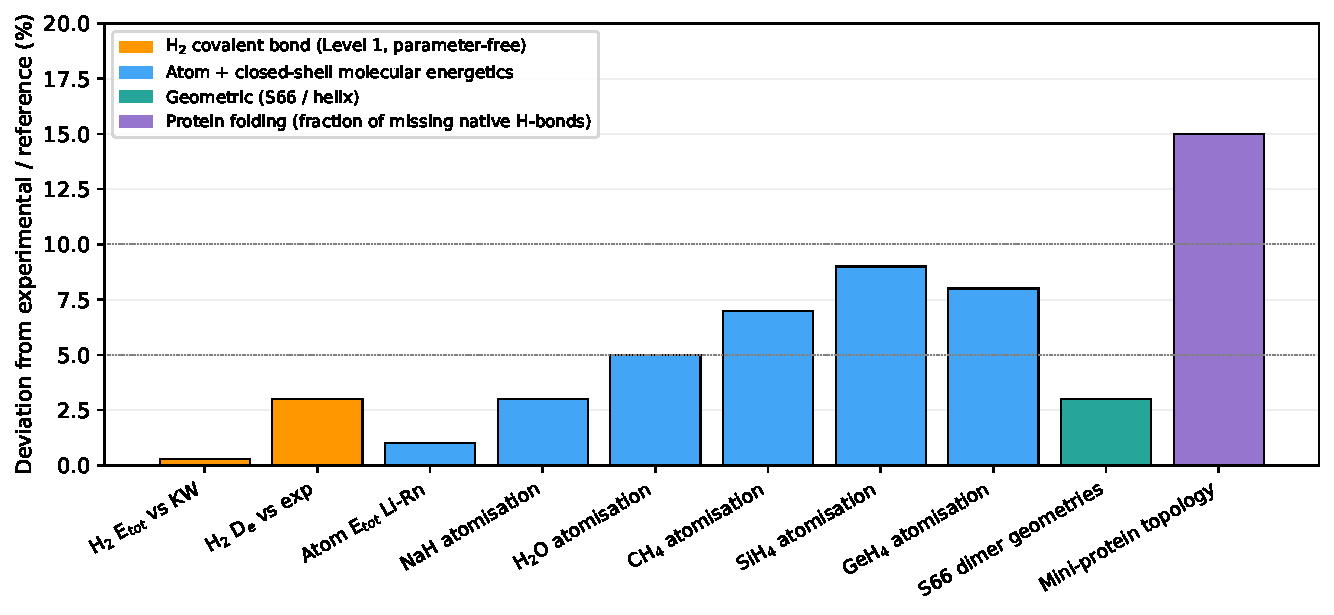
\includegraphics[width=0.95\textwidth]{figures/validation_summary.pdf}
\caption{RealQM validation summary: deviation from experimental reference across regimes. Closed-shell molecular energetics (blue) sit at $\sim$1--10\% across atoms and four periodic-table groups. The foundational H$_2$ covalent bond at parameter-free Level-1 (orange) matches Kolos--Wolniewicz to 0.3\% on total energy and the experimental dissociation energy to 3\%. Geometric matches against CCSD(T) and helix-geometry references (teal) are 3--9\%. Protein-folding deviations (purple) are reported as the fraction of native H-bonds not formed. The NaCl Lindemann-threshold T (red) overshoots experimental $T_m$ by $\sim$50\% due to uncalibrated Brownian-dynamics time mapping; the transition character is qualitatively correct.}
\label{fig:summary}
\end{figure}

\begin{table}[h!]
\centering
\small
\renewcommand{\arraystretch}{1.15}
\begin{tabular}{l l r r l l}
\toprule
\textbf{Regime} & \textbf{System / quantity} & \textbf{RealQM} & \textbf{Reference} & \textbf{Match} & \textbf{Section} \\
\midrule
Atoms (Level 1)        & Total energies, Li--Rn        & ---         & observation     & $\sim$1\%               & \ref{sec:atoms}     \\
\midrule
Covalent bond          & H$_2$ binding energy          & $-112$      & $-109$ kcal/mol & 3\%                     & \ref{sec:h2bond}    \\
\midrule
Group 1 hydride        & NaH atomization                & $-48$       & $-47$           & 2\%                     & \ref{sec:hydrides}  \\
                       & KH atomization                 & $-42$       & $\sim\!-43$     & 2\%                     & \ref{sec:hydrides}  \\
Group 2 hydride        & BeH$_2$ atomization            & $-140$      & $-144$          & 3\%                     & \ref{sec:hydrides}  \\
Group 14 hydride       & CH$_4$ atomization             & $-369$      & $-396$          & 7\%                     & \ref{sec:hydrides}  \\
                       & SiH$_4$ atomization            & $-348$      & $-320$          & 9\%                     & \ref{sec:hydrides}  \\
                       & GeH$_4$ atomization            & $-272$      & $-281$          & 3\%                     & \ref{sec:hydrides}  \\
Group 16 hydride       & H$_2$O atomization             & $-225$      & $-232$          & 3\%                     & \ref{sec:hydrides}  \\
\midrule
Non-covalent dimers    & 5 H-bonded dimers, geometry    & ---         & CCSD(T)         & 1--5\% (distances)      & ---                 \\
\midrule
Reactions              & HF $+$ H$_2$O proton transfer    & H$_t$--O = 0.99 \AA & exp. $\sim$1.0  & qualitative correct  & \ref{sec:reactions} \\
                       & HCl $+$ NH$_3$ proton transfer   & H$_t$--N = 0.97 \AA & exp. $\sim$1.0  & qualitative correct  & \ref{sec:reactions} \\
                       & H $+$ H$_2$ exchange             & symmetric H$_3$ saddle & ---       & qualitative correct & \ref{sec:reactions} \\
\midrule
Protein folding        & 12-Gly $\beta$-hairpin (dry)     & $150^\circ \to 105^\circ$ & folded   & qualitative correct  & \ref{sec:proteins}  \\
                       & 8-Gly $\alpha$-helix             & $r$=2.1 \AA, rise 1.63 \AA & ideal helix & 9\%             & \ref{sec:proteins}  \\
                       & Villin HP35 native H-bonds       & 7 of 9 formed         & native       & 78\%                  & \ref{sec:proteins}  \\
\midrule
Excited states         & Orthohelium ($1s\,2s$, $^3$S)    & directly accessible  & known         & qualitative correct & \ref{sec:orthohelium}\\
\midrule
Materials              & NaCl crystal melt              & T$_\mathrm{sim} \approx 1500$--$2000$~K & $T_m = 1074$~K & 1.4--1.9$\times$ overshoot                & \ref{sec:nacl}     \\
                       & CO$_2$ dry-ice (asymmetric Bernoulli) & T$_\mathrm{sim} \approx 1000$~K  & $T_{\rm sub} = 195$~K  & 5.1$\times$ (~80\% dispersion missing)        & \ref{sec:nacl}     \\
                       & N$_2$ solid (symmetric Bernoulli) & T$_\mathrm{sim} \approx 1000$~K  & $T_{\rm sub} = 60$~K   & 17$\times$ ($\sim$99\% dispersion missing)    & \ref{sec:nacl}     \\
\bottomrule
\end{tabular}
\caption{Summary of validation results. Energies in kcal/mol unless otherwise stated; \% values are deviation of RealQM from reference.}
\label{tab:summary}
\end{table}

The pattern across regimes is consistent: \textbf{within $\sim$1--10\%} for closed-shell molecular energetics where the Level-3 reduction matches the molecular electron count and bonding topology; \textbf{qualitatively correct} for reactive chemistry, protein folding, and excited states; \textbf{$\sim$1.5$\times$ scale offset, transition character correct} for condensed-phase melting where the Brownian-dynamics time mapping is uncalibrated.

\section{Limitations}\label{sec:limitations}

Two regimes lie outside the validation reported here. \textbf{Weak intermolecular interactions} (hydrogen bonds at $\sim$5 kcal/mol $= 0.008$ Ha) are below the model's absolute-energy noise floor of $\sim$0.1 Ha; geometric agreement on S66 dimers is good (1--5\%) but quantitative interaction energies are not reliable. \textbf{Dispersion} (van der Waals interactions between non-polar species) is absent at Level 3 entirely, as the unit-density model has no mechanism for the correlated electron motion that produces vdW. Excited states are accessible (Section~\ref{sec:orthohelium}) but at the present stage have only been validated on the simplest cases.

\section{Stability of Matter}\label{sec:som}

Stability of matter --- the requirement that the total electronic ground-state energy of a system of $N$ atoms be bounded below by an extensive quantity (linear in $N$ rather than diverging more rapidly) --- is among the most fundamental properties demanded of any quantum theory of matter. Without it, bulk matter could not exist.

\paragraph{The standard-QM picture: a deep but difficult proof.}
Within standard quantum mechanics (StdQM) and density functional theory, proving stability of matter has historically been a major mathematical undertaking. \textbf{Dyson and Lenard} gave the first rigorous proof in 1966~\cite{DysonLenard67}, a 26-page paper that Dyson himself characterized as ``awful mathematics''. \textbf{Lieb and Thirring} compressed the proof to three pages in 1975~\cite{LiebThirring75}, then expanded it into the 300-page book \emph{The Stability of Matter in Quantum Mechanics} (2005). The proof's central difficulty stems from the \textbf{global support of electron wavefunctions} in StdQM: in principle, every electron can interact with every nucleus, and intricate book-keeping is required to prevent local accumulation of charge density from driving the potential energy to $-\infty$. The proof is not part of standard textbook treatments of QM, even though stability is a precondition for everything those textbooks describe.

The Lieb--Thirring bound on the ground-state energy of an atom of nuclear charge $Z$ scales as
\begin{equation}
E(Z) \sim -Z^{7/3},
\end{equation}
a result derived from the Thomas--Fermi model rather than the full Schr\"odinger equation.

\paragraph{The RealQM picture: stability follows directly.}
In the multiphase formulation of Section~\ref{sec:reformulation}, stability of matter follows essentially from atomic stability via the \textbf{Hardy inequality}: for any $\psi \in H^1(\mathbb{R}^3)$,
\begin{equation}\label{eq:hardy}
\int \frac{\psi^2(\mathbf{x})}{|\mathbf{x}|} \, d\mathbf{x}
\;\le\;
\Bigl(\int \psi^2(\mathbf{x}) \, d\mathbf{x}\Bigr)^{1/2}
\Bigl(\int |\nabla \psi(\mathbf{x})|^2 \, d\mathbf{x}\Bigr)^{1/2}.
\end{equation}
Used by Kato in his analysis of the Schr\"odinger equation, the inequality bounds the singular Coulomb potential energy at a nucleus by a product of the $L^2$-norm and the kinetic-energy semi-norm of the wavefunction. In RealQM, the total wavefunction $\Psi$ of an atom with nuclear charge $Z$ has unit-density components meeting at the Bernoulli free boundary (continuity plus homogeneous Neumann), with $\Psi \in H^1(\mathbb{R}^3)$ and $\|\Psi\|_2^2 = Z$ (one unit-charge density per electron, $Z$ electrons in a neutral atom). Applying~\eqref{eq:hardy} directly to the global atomic $\Psi$ and optimizing the kinetic--potential balance yields the atomic energy lower bound
\begin{equation}\label{eq:atom-bound}
E_{\rm atom} \;\ge\; -C\, Z^3,
\end{equation}
with $C$ an absolute constant. For a system of $N$ non-overlapping atoms each of charge $Z$, the bounds add to give
\begin{equation}\label{eq:bulk-bound}
E \;\ge\; -C\, N\, Z^3,
\end{equation}
which is the ``stability of the second kind'' of the Dyson--Lenard--Lieb--Thirring tradition: total energy is extensive in $N$, with no possibility of collapse to $-\infty$.

\textbf{The non-overlap constraint is the physical origin of stability in RealQM.} Each atom's potential-energy contribution is controlled by its own kinetic energy through Hardy on its own region of support; no global book-keeping is required because the contributions from distinct atoms simply add. Stability is a direct consequence of the formulation rather than a deep theorem to be proved separately.

\paragraph{Heuristic atomic energy scaling.}
The rigorous Hardy bound~\eqref{eq:atom-bound} establishes stability with $E_{\rm atom} \ge -CZ^3$ but is not tight; the actual ground-state energy of an atom grows more slowly with $Z$. A heuristic estimate within the unit-density formulation can be obtained from an approximate shell structure with shell index $m$: shell radius $r_m \sim m^3/Z$, shell thickness $d_m \sim m^2/Z$, $2m^2$ electrons in the $m$-th filled shell, and charge density $\rho_m(r) \sim Z/r^2$ in spherical symmetry. Integrating kinetic and potential contributions over a density profile of this form produces, at heuristic level, an atomic ground-state energy of order
\begin{equation}
E(Z) \;\sim\; -\log(Z)\, Z^2,
\end{equation}
i.e.\ $-Z^2$ up to a logarithmic correction. The shell-scaling laws above are \emph{heuristic} estimates, not rigorously derived asymptotics, and the resulting $-\log(Z)Z^2$ form is intended only as an order-of-magnitude indication. The Thomas-Fermi--based Lieb--Thirring scaling $-Z^{7/3}$ is a different heuristic prediction; both lie comfortably below the rigorous $-Z^3$ Hardy upper bound on $|E|$ and disagree only at the level of subleading corrections. A precise comparison of the two heuristic scalings, and of either with experimental atom energies across the periodic table, is left for follow-up work.

\paragraph{Significance.}
Stability of matter, viewed in StdQM as one of the deepest theorems of mathematical physics, becomes in RealQM a one-paragraph consequence of the Hardy inequality applied to non-overlapping electronic territories. The contrast is informative: \textbf{the proof difficulty in StdQM is not a feature of the underlying physics but a symptom of the formulation.} Working in $3N$-dimensional configuration space with overlapping orbitals forces the singularities of the Coulomb potential to be controlled globally, requiring the elaborate apparatus of Dyson--Lenard--Lieb--Thirring. Working in real 3D space with non-overlapping unit densities localizes the control, and stability falls out of the variational structure.

The natural pedagogical conclusion is that stability of matter, currently absent from standard QM curricula because the StdQM proof is too difficult, can be presented straightforwardly in the RealQM formulation as an introductory result --- a property of any system of non-overlapping unit electron densities under Coulomb interaction.

\section{An analogous model of the atomic nucleus}\label{sec:nucleus}

The mathematical framework of Section~\ref{sec:reformulation} --- non-overlapping unit charge densities in 3D real space, Coulomb interactions, Bernoulli free boundaries, variational minimization --- is not specific to chemistry. The same multiphase 3D continuum mechanics applies to atomic nuclei when the constituents are taken to be protons and electrons, returning to a pre-1932 picture of nuclear structure.

In this picture a neutron is identified with a proton--electron pair (the proton--electron model that predates the discovery of the neutron as an elementary particle). A stable nucleus with $Z$ protons and $N$ neutrons therefore contains $(Z+N)$ protons and $N$ electrons, with $N \approx Z$ giving roughly twice as many protons as electrons. The simplest non-trivial case is helium-4 ($Z=2$, $N=2$), modeled as 4 protons and 2 electrons.

\paragraph{The model.}
The setup uses the same multiphase formulation:
\begin{itemize}
\item 4 unit-charge densities representing protons (each $+1$);
\item 2 unit-charge densities representing electrons (each $-1$);
\item Each density supported on its own non-overlapping spatial region in $\mathbb{R}^3$, with continuity and homogeneous Neumann at the inter-species Bernoulli interface;
\item Coulomb interactions, signed appropriately for the charges: opposite-sign attractive, same-sign repulsive;
\item Per-domain mass: the kinetic-energy operator coefficient is $\propto 1/m_i$, distinguishing the heavy proton from the light electron;
\item No external confining potential.
\end{itemize}

The energy functional is the standard Coulomb sum
\begin{equation}
E = T_p + T_e + V_{ee} + V_{pp} + V_{ep},
\end{equation}
with $T_p = \tfrac{1}{2 m_p} \sum_a \int |\nabla \sqrt{\rho_a^{(p)}}|^2 d\mathbf{r}$ for the protons (mass-weighted) and $T_e$ analogous for the electrons. The minimum is taken over all the densities and over the boundary location between the inner electron core and the outer proton shell.

\paragraph{Mutual confinement.}
In the standard nuclear shell model, protons and neutrons sit in an effective potential approximating the average force from all other nucleons. Here there is no such external potential. The 4 protons confine the 2 electrons through their collective $+4$ Coulomb attraction; in turn, the 2 electrons confine the protons through their collective $-2$ Coulomb attraction. The electrons need the protons to be confined, and the protons need the electrons to be confined. Numerical experiment confirms that with only \emph{1} electron ($-1$ against $+4$) the attraction is too weak --- the proton shell disintegrates outward. With \emph{2} electrons the system stabilizes. The textbook 2:1 proton-to-electron ratio of stable nuclei ($N \approx Z$) emerges as a binding requirement of mutual confinement.

\paragraph{Result for He-4.}
Energy minimization at fixed boundary radius $R$ between the inner electron core and the outer proton shell, swept across $R$, reveals a clear binding minimum. The protons localize in an outer shell with their density peaked at the boundary; the electrons localize in an inner core. The two species are sharply separated by the Bernoulli interface, with the boundary position selected by the variational principle (continuity plus homogeneous Neumann across the boundary, as in the chemistry sections). The binding character --- mutual confinement, sharp species separation, stable equilibrium $R$ --- is qualitatively consistent with helium-4 being the most tightly bound of the small nuclei. Quantitative agreement with experimental nuclear binding energies is not the goal at this exploratory stage; the framework reproduces the proton--electron model's qualitative predictions through the same RealQM machinery developed for chemistry.

\paragraph{Significance.}
The nuclear extension is reported here as a side step from the main paper. Its purpose is to demonstrate that the mathematical framework --- multiphase non-overlapping unit densities in real 3D space, with Bernoulli free boundaries and pure Coulomb interactions --- is applicable to atomic-scale physics quite generally. The chemistry validation of Section~\ref{sec:validation} is therefore one application of a broader continuum-mechanics formulation; the nuclear model is another. The framework provides a unifying mathematical structure spanning at least two scales of physics through a single variational-Coulomb-with-Bernoulli-boundary principle. Whether quantitative agreement with nuclear-binding observables can be obtained, and whether the proton--electron picture can be extended beyond He-4 to heavier stable nuclei, are questions for follow-up work.

\section{Chemistry vs Physics}\label{sec:chemvphys}

A central question in the philosophy of chemistry is whether \textbf{(A)} chemistry can be explained by quantum physics, as \textbf{Dirac famously claimed in 1929 at the birth of quantum mechanics}, or \textbf{(B)} something more is required, as has been argued by leading chemists for nearly a century. Position (B) is the view that chemistry possesses an irreducible conceptual content --- orbitals, bonds, valence, hybridisation, electronegativity --- that does not follow from Schr\"odinger's equation alone, no matter how many computational resources are thrown at it. Position (A) is the view that chemistry \emph{is} applied quantum physics, and that the apparent autonomy of chemical concepts is an artefact of the practical impossibility of solving the underlying equations.

The hundred-year stalemate has been driven less by disagreement on principle than by the fact that, within the standard $3N$-dimensional wavefunction formulation that Dirac himself had in mind in 1929, the equations are indeed unsolvable for any system of chemical interest without approximations whose chemistry-specific character (basis sets, exchange--correlation functionals, fitted force fields) seems to vindicate position (B).

RealQM provides \textbf{concrete evidence that Dirac's position (A) was correct, although not within the 1929 wavefunction-on-$3N$-space formulation that Dirac himself proposed}. The reformulation as a system of non-overlapping unit electron densities in real 3D space, with energy minimization over Coulomb interactions alone, recovers atoms (Section~\ref{sec:atoms}), the covalent bond and its He limit (Section~\ref{sec:h2bond}), atomization energies of hydrides across periodic-table groups (Section~\ref{sec:hydrides}), reactive chemistry (Section~\ref{sec:reactions}), and protein folding (Section~\ref{sec:proteins}) --- using only physics, with no chemistry-specific empirical input beyond the kernel parameters that encode the level-by-level reduction. Chemistry emerges as the variational principle's response to multiple nuclei being present, with no separate machinery required.

The conclusion we draw is not that the standard $3N$-dimensional formulation should be abandoned --- for high-precision spectroscopy, transition probabilities, and excited-state dynamics it remains the canonical tool --- but that \textbf{chemistry-as-applied-physics is achievable} when one is willing to reformulate the problem in real 3D space with an appropriate non-overlap constraint. Dirac was right; the equations were just being written in the wrong space.

\section{The collaboration as part of the contribution}\label{sec:collaboration}

The mathematical reformulation in Section~\ref{sec:reformulation} and the hierarchy of Levels 1--4 are the work of the human author. They predate the AI collaboration and have been developed over a decade of independent work. The author also wrote the initial p5.js prototype simulations that established the numerical core (real-space grid, ITP, Poisson solver, basic visualization) used as the starting point for the WebGPU implementation. The full WebGPU port, the validation suite, the systematic kernel-architecture sweeps reported in Section~\ref{sec:validation}, and the curated public Gallery were developed from those starting templates through extended collaboration with \textbf{Claude}, an AI code assistant produced by Anthropic.

We document the pattern of the collaboration here because we believe it is a worth-reporting example of how a single mathematical mind can produce research-grade interactive scientific software with an AI engineering partner.

The human posed mathematical and chemical questions: ``What if the model uses $Z=2$ instead of $Z=4$ for carbon?'' ``Does the H-bond force correctly point toward the acceptor lone pair?'' ``Why does this geometry prefer stretched over bonded?'' The AI translated these into runnable simulations, identified bugs in real time, ran systematic parameter sweeps, computed and tabulated results, drafted candidate gallery cards, and challenged claims that did not survive scrutiny.

The interaction was iterative and surprisingly productive: a question asked at 9:00 might be answered with a working scan file at 9:05, partial results at 9:30, a full sweep table at 10:00, and a refined analysis incorporating the latest data by 10:30. Across many such cycles, the validation table reported in Section~\ref{sec:validation} was assembled.

We also record honestly where the AI's interpretations needed correction. Several times the AI prematurely concluded that a result was ``within $X\%$ of experiment'' before convergence had been confirmed; in each case the human pushed back and the AI revised. The Gallery's ``Assessment by Claude'' card reflects this --- its caveats were rewritten more than once during the project as the evidence accumulated.

We find that the right framing for the collaboration is \textbf{mathematical mind + AI engineering partner}: the human supplies the theory, the questions, the chemical intuition, and the standards for what counts as evidence; the AI supplies the implementation, the systematic exploration, and the speed. Neither could have produced this result alone in any reasonable timeframe.

\section{Code and reproducibility}\label{sec:code}

The full RealQM implementation, including the validation suite, the systematic kernel-architecture sweeps reported in Section~\ref{sec:validation}, and the curated public Gallery, is available at:

\begin{itemize}
\item \textbf{Code repository:} \url{https://github.com/Claes542/RealMolecule}
\item \textbf{Interactive Gallery:} \url{https://claes542.github.io/RealMolecule/gallery.html}
\item \textbf{RealQM project site:} \url{https://physicalquantummechanics.blogspot.com}
\item \textbf{Author's blog:} \url{https://claesjohnson.blogspot.com}
\item \textbf{Browser requirements:} Chrome 113+, Edge 113+, or Safari 17+ (WebGPU)
\item \textbf{Hardware:} any modern integrated or discrete GPU ($\sim$1 GB GPU memory for $\sim$200$^3$ grid)
\end{itemize}

All results in this paper can be reproduced by opening the relevant \texttt{.html} files in the repository. Each binding-energy data point in Section~\ref{sec:validation} corresponds to a specific URL parameterization ($R$, $r_c$) of a specific scan file (e.g., \texttt{mol\_fast\_H4X\_Z2\_scan.html?R=1.0\&rc=0.2}). The Gallery's ``Kernel Splitting'' and ``Periodic-Table Coverage'' cards link directly to the scan files used to generate the reported numbers.

We deliberately do not include figures in this preprint. The Gallery contains many interactive visualizations --- density slices, 3D molecular views, force-arrow displays, real-time dynamics --- that are far more informative as live simulations than as static images. Readers wishing to inspect electron densities, watch molecules relax, or run their own kernel-architecture sweeps should consult the Gallery directly.

\section*{Acknowledgments}

The author is very happy to meet Claude Code in a fruitful cooperation way beyond initial expectations after lonely struggle with coding over long time.

\section*{Competing interests}

None declared.

\begin{thebibliography}{9}

\bibitem{HK64}
P.~Hohenberg and W.~Kohn,
\emph{Inhomogeneous electron gas},
Phys.\ Rev.\ \textbf{136}, B864 (1964).

\bibitem{KS65}
W.~Kohn and L.~J.~Sham,
\emph{Self-consistent equations including exchange and correlation effects},
Phys.\ Rev.\ \textbf{140}, A1133 (1965).

\bibitem{MHG17}
N.~Mardirossian and M.~Head-Gordon,
\emph{Thirty years of density functional theory in computational chemistry: an overview and extensive assessment of 200 density functionals},
Mol.\ Phys.\ \textbf{115}, 2315 (2017).

\bibitem{Bader90}
R.~F.~W.~Bader,
\emph{Atoms in Molecules: A Quantum Theory},
Oxford University Press (1990).

\bibitem{Ruedenberg62}
K.~Ruedenberg,
\emph{The physical nature of the chemical bond},
Rev.\ Mod.\ Phys.\ \textbf{34}, 326 (1962).

\bibitem{Kutzelnigg90}
W.~Kutzelnigg,
\emph{The physical mechanism of the chemical bond},
Angew.\ Chem.\ Int.\ Ed.\ \textbf{12}, 546 (1973).

\bibitem{Lindemann10}
F.~A.~Lindemann,
\emph{\"Uber die Berechnung molekularer Eigenfrequenzen},
Phys.\ Z.\ \textbf{11}, 609 (1910).

\bibitem{BornMayer32}
M.~Born and J.~E.~Mayer,
\emph{Zur Gittertheorie der Ionenkristalle},
Z.~Phys.\ \textbf{75}, 1 (1932).

\bibitem{Shaw10}
D.~E.~Shaw \emph{et al.},
\emph{Atomic-level characterization of the structural dynamics of proteins},
Science \textbf{330}, 341 (2010).

\bibitem{DysonLenard67}
F.~J.~Dyson and A.~Lenard,
\emph{Stability of matter, I},
J.\ Math.\ Phys.\ \textbf{8}, 423 (1967).

\bibitem{LiebThirring75}
E.~H.~Lieb and W.~E.~Thirring,
\emph{Bound for the kinetic energy of fermions which proves the stability of matter},
Phys.\ Rev.\ Lett.\ \textbf{35}, 687 (1975).

\end{thebibliography}

\end{document}
